\documentclass[tikz, border=10pt]{standalone}
\usepackage{pgfplots}
\usepgfplotslibrary{fillbetween}
\usepgfplotslibrary{groupplots}
\pgfplotsset{compat=1.18}

\begin{document}
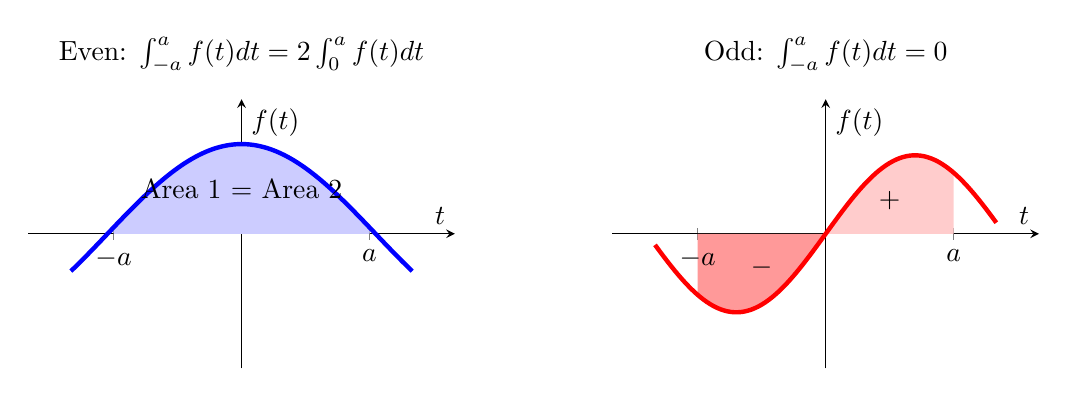
\begin{tikzpicture}
    \begin{groupplot}[
        group style={
            group size=2 by 1,
            horizontal sep=2cm
        },
        width=7cm, height=5cm,
        axis lines=middle,
        xlabel={$t$}, ylabel={$f(t)$},
        xmin=-2.5, xmax=2.5,
        ymin=-1.2, ymax=1.2,
        xtick={-1.5, 0, 1.5},
        xticklabels={$-a$, 0, $a$},
        ytick=\empty,
        samples=100,
        domain=-2:2
    ]
        % (a) Even Function
        \nextgroupplot[title={Even: $\int_{-a}^{a} f(t)dt = 2\int_{0}^{a} f(t)dt$}]
        \addplot[name path=f, blue, ultra thick] {0.8*cos(deg(x))};
        \path[name path=axis] (axis cs:-1.5,0) -- (axis cs:1.5,0);
        \addplot[fill=blue!20] fill between[of=f and axis, soft clip={domain=-1.5:1.5}];
        \node at (axis cs:0, 0.4) {Area 1 = Area 2};
        
        % (b) Odd Function
        \nextgroupplot[title={Odd: $\int_{-a}^{a} f(t)dt = 0$}]
        \addplot[name path=g, red, ultra thick] {0.7*sin(deg(1.5*x))};
        \path[name path=axisg] (axis cs:-1.5,0) -- (axis cs:1.5,0);
        \addplot[fill=red!20] fill between[of=g and axisg, soft clip={domain=0:1.5}];
        \addplot[fill=red!40] fill between[of=g and axisg, soft clip={domain=-1.5:0}];
        \node at (axis cs:0.75, 0.3) {$+$};
        \node at (axis cs:-0.75, -0.3) {$-$};
    \end{groupplot}
\end{tikzpicture}
\end{document}
